\documentclass[twoside,12pt,fleqn,a4paper]{book}
\renewcommand{\figurename}{Figura}
\usepackage{calc}
\usepackage{color}
\usepackage{ulem}
\setlength{\topmargin}{-1cm}
\setlength{\textwidth}{16.cm}
\setlength{\textheight}{23.5cm}
\setlength{\oddsidemargin}{0.3cm}
\setlength{\evensidemargin}{210mm-2in-\oddsidemargin-\textwidth}
\sloppy
\usepackage{indentfirst}
\usepackage{amsfonts}
\usepackage{amssymb}
\usepackage{amsmath}
\usepackage{graphicx}
\usepackage{caption}
\usepackage{subcaption}
\usepackage{afterpage}
\usepackage{bm}
%\usepackage[usenames]{color}
\usepackage{lastpage}
%\usepackage[numbib,nottoc]{tocbibind}
\usepackage{fancyhdr}
\usepackage{braket}
%\usepackage[sectionbib]{chapterbib}
\usepackage[hyperindex,breaklinks=true]{hyperref}

\usepackage{tikz}  %TikZ central library is called.
\usepackage{tcolorbox}
\usetikzlibrary{automata,positioning} % automata and positioning libraries are required to use nodes and coordinates in addition to placement propetries.


\pagestyle{empty}

\renewcommand{\chaptername}{\Large{Capitolul}}

\renewcommand{\appendixname}{\Large{Anexa}}

\renewcommand{\contentsname}{\Large{Cuprins}}

\renewcommand{\bibname}{\Large{Bibliografie}}



\begin{document}
\clearpage{\pagestyle{empty}\cleardoublepage}

\pagestyle{empty}

\begin{center}
\begin{Large}
Universitatea din Bucure\c sti, Facultatea de Fizic\u a
\end{Large}
\end{center}
\vspace*{5cm}

\begin{center}
\begin{Large}
{\bf Elemente de teoria ciocnirilor la energii joase}
\end{Large}
\end{center}

\begin{center}
-Lucrare de licen\c{t}\u{a}-
\end{center}

\vspace*{7cm}

\begin{large}
Absolvent  	 \hfill Coordonator \c{s}tiin\c{t}ific \hspace*{1.5cm}

Pan\u{a} Gabriel Tiberiu\hfill Conferen\c tiar M\u{a}d\u{a}lina Boca
\end{large}

\vfill

\begin{center}


Sesiunea Iunie 2019

\end{center}
\clearpage{\pagestyle{empty}\cleardoublepage}

\setcounter{page}{1}
\renewcommand{\thepage}{\roman{page}}

\pagestyle{plain}

\tableofcontents
\clearpage{\pagestyle{empty}\cleardoublepage}

%\listoffigures
%\clearpage{\pagestyle{empty}\cleardoublepage}

%\listoftables
%\clearpage{\pagestyle{empty}\cleardoublepage}

\renewcommand{\thepage}{\arabic{page}}

\setcounter{page}{1}

%\pagestyle{fancy}
%\renewcommand{\chaptermark}[1]{\markboth{#1}{}}
%\renewcommand{\sectionmark}[1]{\markright{#1}}
%\fancyhead[LO]{\bfseries\nouppercase\leftmark}
%\fancyhead[RO]{\bfseries\thepage}%\ / \pageref{LastPage}}
%\fancyhead[RE]{\bfseries\nouppercase\rightmark}
%\fancyhead[LE]{\bfseries\thepage}%\ / \pageref{LastPage}}
%\fancyfoot{}



%\pagestyle{fancy}
%\renewcommand{\chaptermark}[1]{\markboth{#1}{}}
%\renewcommand{\sectionmark}[1]{\markright{#1}}

%\fancyhead[LO]{\bfseries\nouppercase\leftmark}
%\fancyhead[RO]{\thepage}%\ / \pageref{LastPage}}
%\fancyhead[RE]{\bfseries\nouppercase\leftmark}%{\bfseries\nouppercase\rightmark}
%\fancyhead[LE]{\thepage}%\ / \pageref{LastPage}}
%\fancyfoot{}



\chapter{Introducere}

Ciocnirile dintre particule la energii joase \c{s}i ultra-joase ocup\u{a} un loc strategic la interesec\c{t}ia mai multor subiecte de cercetare \^{i}n chimia fizic\u{a}, \^{i}n fizica atomic\u{a}, molecular\u{a}, optic\u{a} \c{s}i  fizica st\u{a}rii condensate. Natura acestor ciocniri are un impact esen\c{t}ial \^{i}n studiul proceselor ce au loc la scar\u{a} atomic\u{a}, dintre care enumer\u{a}m: manipularea optic\u{a} a proceselor inelastice si reactive, m\u{a}surarea cu precizie a parametrilor atomici \c{s}i moleculari, coeren\c{t}ele materie-und\u{a} \c{s}i statistica condensa\c{t}ilor cuantici forma\c{t}i din atomi ce interac\c{t}ioneaz\u{a} slab. Aceste c\^{a}teva exemple sunt suficiente pentru a justifica interesul  \^{i}n studiul ciocnirilor la energii joase.\\


\^{I}n procesul de r\u{a}cire a gazelor p\^{a}n\u{a} la temperaturi foarte joase abilitatea de a controla interac\c{t}iunile dintre atomii gazului respectiv este esen\c{t}ial\u{a}. Cu c\^{a}t densitatea scade, cu atat interac\c{t}iile de dou\u{a} corpuri (doi atomi) devin predominante \c{s}i ele pot fi descrise \^{i}n termeni de ciocniri. \^{I}n lucrarea de fa\c{t}\u{a} ne vom ocupa de ciocnirile elastice dintre atomi. Acestea sunt esen\c{t}iale pentru atingerea echilibrului termic.\\

La temperaturi foarte joase, descrierile ce folosesc  teoria c\^{a}mpului mediu  ale gazelor cuantice degenerate depind de un num\u{a}r foarte mic de parametri de ciocnire. De exemplu, forma \c{s}i dinamica condensatelor Bose-Einstein depind doar de lungimea de \^{i}mpr\u{a}\c{s}tiere, definit\u a \^{\i}n cadrul teoriei ciocnirilor.\\

Trebuie men\c{t}ionat faptul c\u{a} este posibil de controlat interac\c{t}ia atom-atom \c{s}i prin rezonan\c{t}e Feshbach, pe care le putem observa prin calculul defazajelor.\\

\^{I}n aceas\u{a} lucrare vom calcula defazajele, apoi lungimea de \^{i}mpr\u{a}\c{s}tiere \^{i}n limita de energie zero pentru c\^{a}teva poten\c{t}iale simple, apoi pentru un poten\c{t}ial de interac\c{t}ie aproximat penru ciocnirile atomilor de Cesiu. Acesta con\c{t}ine dou\u{a} p\u{a}r\c{t}i: o component\u{a} de raz\u{a} scurt\u{a} ce dispare la o anumit\u{a} lungime \c{s}i o component\u{a} ce const\u{a} \^{i}ntr-o superpozi\c{t}ie de termeni Van der Waals.\\

%Realiz\u{a}m calculul \c{t}in\^{a}nd cont c\u{a} exist\u{a} solu\c{t}ii analitice pentru ecua\c{t}iile Schr\"{o}dinger radiale la energie nul\u{a} pentru poten\c{t}iale simple, folosite \^{i}n fizica atomic\u{a}, deci contribu\c{t}iile lungimilor de \^{i}mpr\u{a}\c{s}tiere pot fi g\u{a}site exact. A\c{s}adar putem g\u{a}si acest parametru \c{s}i pentru un poten\c{t}ial mai complex, apropiat de realitate.


Structura tezei este urm\u atoarea: \^{\i}n capitolul 2 prezent\u am elemente de teoria ciocnirilor \^{\i}n mecanica clasic\u a \c si \^{\i}n fizica cuantic\u a. Discut\u am solu\c tia de \^{\i}mpr\u a\c stiere, modul de ob\c tinere a acesteia  cu ajutorul fun\c tiei Green, aproxima\c tia Born, descompunerea solu\c tiei  de \^{\i}mpr\u a\c stiere \^{\i}n unde par\c tiale \c si \^{\i}n final definirea defazajelor \c si a lungimii de \^{\i}mpr\u a\c stiere. In capitolul 3 prezent\u a exemple numerice pentru c\^ateva poten\c tiale model;  metoda numeric\u a se bazeaz\u a pe un cod scris in Mathematica, ce este prezentata \^{\i}n anexa B. Anexa A con\c tine propriet\u a\c ti ale func\c tiilor Bessel sferice.




%%% Local Variables:
%%% mode: latex
%%% TeX-master: "../RE"
%%% End:

\clearpage{\pagestyle{empty}\cleardoublepage}

\input{ch2_elem_teoria_ciocnirilor/ch2_elem_teoria_ciocnirilor.tex}
\clearpage{\pagestyle{empty}\cleardoublepage}
\chapter{Rezultate numerice}

\section{Lungimea de \^{i}mpr\u{a}\c{s}tiere pentru c\^{a}teva poten\c{t}iale simple }
Dup\u{a} cum am ar\u{a}tat mai sus, pentru energii joase, coliziunile sunt, \^{i}n esen\c{t}\u{a} \^{i}n regimul de und\u{a} s, adica corespund unei unde \^{i}mpr\u{a}\c{s}tiate izotropic. Mai mult, c\^{a}nd vectorul de und\u{a} relativ $k$ (sau energia $\hbar^2k^2/(2m_r)$) tinde la zero, defazajul $\delta_0(k)$ pentru unda s este propor\c{t}ional cu $k$ (modulo $\pi$) astfel c\u{a} amplitudinea de \^{i}mpr\u{a}\c{s}tiere tinde la o constant\u{a}:
\begin{align}
f(k)\bigg\rvert_{\text{und\u{a} s}}=\frac{e^{i\delta_0k}\sin\delta_0(k)}{k}\to -a \qquad \text{c\^{a}nd} \quad k\to 0 
\end{align}
Solutia problemei de \^{i}mpr\u{a}\c{s}tiere la energii ultra-joase se rezum\u{a} la determinarea unei singure cantit\u{a}\c{t}i: lungimea de \^{i}mpr\u{a}\c{s}tiere $a$.\\

O astfel de determinare se realizeaz\u{a} \^{i}n felul urm\u{a}tor: Scriem ecua\c{t}ia radial\u{a} 
\begin{align}
&\chi''({\bm r})+(\frac{2M}{\hbar^2}(E({\bm k})-U({\bm r}))-\frac{l(l+1}{r^2})\chi({\bm r})=0\label{srad}
\end{align}
pentru $l=0$, pe care o vom integra pe intervalul $r\in (\epsilon,r_{Max})$, unde $\epsilon$ este ales foarte mic, iar $r_{Max}$ este mai mare dec\^at raza de ac\c tiune a potentialului, folosind condi\c tiile la limit\u a
\begin{align}
 &\chi(\epsilon)=\epsilon^{l+1},\quad \chi'(\epsilon)=(l+1)\epsilon^l
\end{align}
Deoarece pentru $r>r_{Max}$ solu\c tia poate fi scris\u a ca o combina\c tie de func\c tii Bessel sferice (Anexa \ref{anexa-bessel}) :
 \begin{align}
&\chi(r_{Max})=A s_l(r_{Max}) +B c_l(r_{Max})\label{eq1}\\
&\chi'(r_{Max})=A s_l'(r_{Max}) +B c_l'(r_{Max})\label{eq2}
\end{align}
unde $s_l(r_{Max})=r_{Max}j_0(k r_{Max})$ \c{s}i $c_l(r_{Max})=r_{Max} y_0 (k r_{Max})$
Putem rezolva sistemul \c{s}i ob\c{t}inem valori pentru constantele $A$ \c{s}i $B$, deci afl\u{a}m $\tan\delta_l=-B/A$. \^{I}n final ob\c{t}inem lungimea de \^{i}mpr\u{a}\c{s}tiere $a$ duc\^{a}ndu-l pe $k$ la zero:
\begin{align}
a=-\lim_{k\to 0}\frac{\tan\delta_0(k)}{k}
\end{align} 
In toate exemplele numerice prezentate \^{i}n continuare vom folosi sistemul de unit\u{a}\c{t}i atomice.

\subsection{Treapta de poten\c{t}ial}

Primul exemplu discutat aici este treapta de poten\c{t}ial, modelat\u{a} de func\c{t}ia:
\begin{align}
V({\bm r})=V(0)\tanh{\frac{{\bm r}-r_0}{\alpha_0}}-V(0)
\end{align}
unde $\alpha_0$ controleaz\u{a} rotunjirea treptei, iar $r_0$ este raza de ac\c{t}iune \c{s}i am ales $M =10^3$ 

Reprezent\u am grafic m\u arimea $-\tan(\delta_0)/k$ ca fun\c tie de $k$ ]c si din grafic putem observa lungimea de \^{\i}mpr\u a\c tiere.
\begin{figure}[h]
\centering
\begin{subfigure}{.5\textwidth}
  \centering
  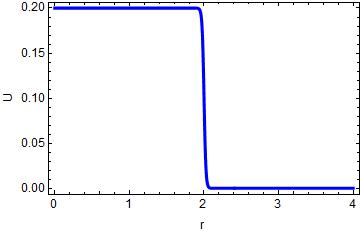
\includegraphics[width=0.9\linewidth]{PotentialTreapta}
  \caption{Poten\c{t}ial Treapt\u{a}}
  \label{fig:sub311}
\end{subfigure}%
\begin{subfigure}{.5\textwidth}
  \centering
  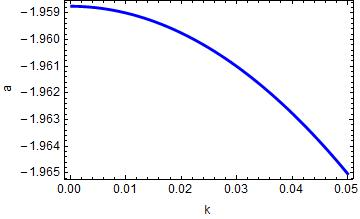
\includegraphics[width=0.9\linewidth]{LungimeImprastiereTreapta}
  \caption{$-\tan(\delta_0)/k$}
  \label{fig:sub312}
\end{subfigure}
\caption{Treapta de poten\c{t}ial}
\label{fig:treapta}
\end{figure}


\subsection{Groapa de poten\c{t}ial}
Al doilea exemplu este groapa de poten\c{t}ial, similar\u{a} cu treapt\u{a}, modelat\u{a} prin aceea\c{s}i func\c{t}ie luat\u{a} cu minus: 
\begin{align}
V({\bm r})=-V(0)\tanh{\frac{{\bm r}-r_0}{\alpha_0}}+V(0)
\end{align}
valorile parametrilor au fost p\u{a}strate
\begin{figure}[h]
\centering
\begin{subfigure}{.5\textwidth}
  \centering
  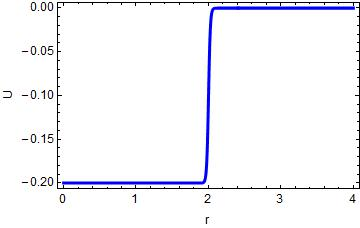
\includegraphics[width=0.9\linewidth]{PotentialGroapa}
  \caption{Poten\c{t}ial Groap\u{a}}
  \label{fig:sub321}
\end{subfigure}%
\begin{subfigure}{.5\textwidth}
  \centering
  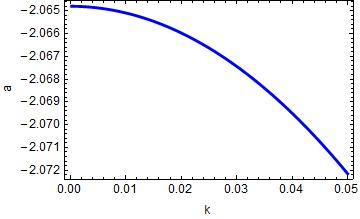
\includegraphics[width=0.9\linewidth]{LungimeImprastiereGroapa}
  \caption{$-\tan(\delta_0)/k$}
  \label{fig:sub322}
\end{subfigure}
\caption{Groapa de poten\c{t}ial}
\label{fig:groapa}
\end{figure}


\subsection{Poten\c{t}ial de tip Van der Waals}
Ultimul exemplu simplu discutat aici este pote\c{t}ialul de tip Van der Waals, modelat de func\c{t}ia:
\begin{align}
U({\bm r})=U(0)\left(\left(\frac{r_0}{{\bm r}}\right)^12-2\left(\frac{r_0}{{\bm r}}\right)^6\right), \qquad \text{unde } U(0)=10^{-6}
\end{align}

\begin{figure}[h]
\centering
\begin{subfigure}{.5\textwidth}
  \centering
  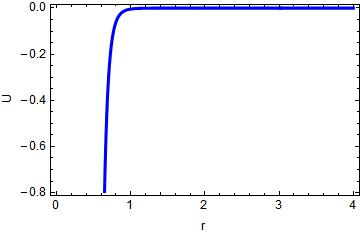
\includegraphics[width=0.9\linewidth]{PotentialVanDerWaals}
  \caption{Poten\c{t}ial de tip Van der Waals}
  \label{fig:sub331}
\end{subfigure}%
\begin{subfigure}{.5\textwidth}
  \centering
  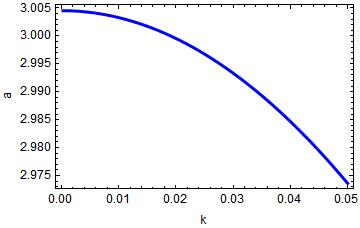
\includegraphics[width=0.9\linewidth]{LungimeImprastiereVanDerWaals}
  \caption{$-\tan(\delta_0)/k$}
  \label{fig:sub332}
\end{subfigure}
\caption{Poten\c{t}ial de tip Van der Waals}
\label{fig:groapa}
\end{figure}


\section{Poten\c{t}ial aproximat pentru atomi de Cs}

Pentru a realiza calculul numeric al defazajelor \^{i}n und\u{a} s \c{s}i a lungimilor de \^{i}mpr\u{a}\c{s}tiere adopt\u{a}m urm\u{a}toarea expresie a poten\c{t}ialului pentru interac\c{t}ia atomilor de Cs:
\begin{align}
U(r)=\frac{1}{2}Br^\alpha e^{-\beta r}-\left(\frac{C_6}{r^6}+\frac{C_8}{r^8}+\frac{C_{10}}{r^{10}}\right)f_c(r)\label{vcs}
\end{align}
Primul termen de dup\u{a} egal reprezint\u{a} repulsia dintre electronii de valen\c{t}\u{a}, iar al doilea reprezint\u{a} suma termenilor Van der Waals, \^{i}nmul\c{t}it\u{a} cu o func\c{t}ie de cutoff $f_c(r)$, ce are rolul de a anula divergen\c{t}a $1/r^n$ la distan\c{t}e mici.\\
Func\c{t}ia de cutoff are forma:
\begin{align}
f_c(r)=\Theta(r-r_c)+\Theta(r_c-r)e^{-(rc/r-1)^2},
\end{align}
unde $\Theta(x)$ reprezint\u{a} func\c{t}ia Heaviside ($\Theta(x)=1,\quad x>0$ \c{s}i $\Theta(x)=0,\quad x<0$)
Parametrii poten\c{t}ialului au fost ale\c{s} din literatur\u{a} \cite{art-VW} (date \^{i}n unit\u{a}\c{t}i atomice):
\begin{center}
 \begin{tabular}{||c c c c c c c||} 
 \hline
 B & $\alpha$ & $\beta$ & $C_6$ & $C_8$ & $C_{10}$ & $r_c$ \\ [0.5ex] 
 \hline 
 0.0016 & 5.53 & 1.072 & 7020 & $1.1 \times 10^6$ & $1.7 \times 10^8$ & 23.165 \\ 
  \hline
\end{tabular}
\end{center}

Situa\c tia este diferit\u a  \^{\i}n acest  caz; un grafic al poten\c tialului
\begin{figure}[h]
  \centering
  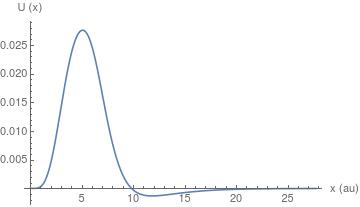
\includegraphics[scale = 0.8]{CS.jpg}
  {\caption{Potentialul (\ref{vcs})\label{gvcs}}}
  \end{figure}
  face u]c sor de \^{\i}n\c teles c\u a prezen\c ta barierei inatl\u a \c si larg\u a faca ca la energii mici propagarea solu\c tiei ``pe sub barier\u a'' sa duc\u a la pierderea complet\u a a preciziei.
  De exemplu \^{\i}n figura \ref{figpsi} este reprezentat\u a solu\c tia $\chi(r)$ g\u asit\u a cu Mathematica pentru $k=0.05$ u.a. E evident c\u a solu\c tia nu are comportarea corect\u a la distan\c te mari.
\begin{figure}[h]
  \centering
  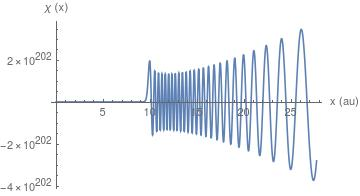
\includegraphics[scale = 0.8]{FIG.jpg}
  {\caption{Potentialul (\ref{vcs})\label{figpsi}}}
  \end{figure}

  
In acest caz sunt mai potrivite metode de evaluare a defazajului bazate pe aproxima\c tia JWKB sau pe calculul direct al fazei solu\c tiei radiale, cum ar fi \cite{ris}, care furnizeaz\u a rezultate in acord cu cele din \cite{art-VW}. 



 

%%% Local Variables:
%%% mode: latex
%%% TeX-master: "../RE"
%%% End:

\clearpage{\pagestyle{empty}\cleardoublepage}
%\chapter{Concluzii}

In concluzie am f\u acut ....

Dupa cum am vazut in ecuatia (\ref{ecs})
%\clearpage{\pagestyle{empty}\cleardoublepage}



\appendix


\input{appendix1/fctBessel.tex}

\clearpage{\pagestyle{empty}\cleardoublepage}

\chapter{Algoritmul si codul numeric}

Algoritmul numeric const\u a \^{\i}n rezolvarea, in Mathematica a ecua\c tiei Schr\"odinger radial\u a (\ref{srad})  cu condi\c tii la limit\u a
\begin{align}
  \chi(r)\mathop{\sim}_{r\rightarrow 0}r^{l+1},\quad 
  \chi'(r)\mathop{\sim}_{r\rightarrow 0}(l+1)r^{l}
\end{align}
\c si calcul derivatei logaritmice la o distan\c t\u a destul de mare (dincolo de raza de ac\c tiune a poten\c tialului). Cu expresia derivatei logaritmice rezolv\u am sistemul (\ref{eq1}-\ref{eq2}) pentru a determina $\tan\delta_l$. Pentru $l=0$ \c si in limita de energii mici determin\u am lungimea de \^{\i}mpr\u a\c stiere.

Codurile Mathematica sunt listate \^{\i}n continuare.
%%% Local Variables:
%%% mode: latex
%%% TeX-master: "../RE"
%%% End:


\clearpage{\pagestyle{empty}\cleardoublepage}


\begin{thebibliography}{1000}
\bibitem{art-VW}G. F. Gribakin, V. V. Flambaum, Phys. Rev. A {\bf 48}, 546 (1993).

\bibitem{Zettili}Nouredine Zettili, Quantum Mechanics Concepts and Aplications, 2nd ed

\bibitem{varenna}Jean Dalibard, Collisional dynamics of ultra-cold atomic gases

\bibitem{Szmytk}Radoslaw Szmytkowski, Analytical calculations of scattering lenghths in atomic physics, J. Phys. A: Math. Gen. 28 (1995) 7333-7345
  
\bibitem{IHP-2007}Claude Cohen-Tannoudji. Atom-atom interactions in ultracold gases. DEA. Institut Henri Poincar\`{e}, 25 et 27 Avril 2007, 2007. $<$ cel-00346023 $>$

\bibitem{Jullienne-RMP-ColdCollisions}John Weiner, V. S. Bagnato, S. Zilio, Paul S. Jullienne, Rev. Mod. Phys, Vol 71, No. 1, January 1999

\bibitem{ris}H. Ouerdane, M. Jamieson, D. Vranceanu and M. Cavagnero, J. Phys. B  {\bf 36}, 4075 (2005).

\end{thebibliography}

%%% Local Variables:
%%% mode: latex
%%% TeX-master: "../RE"
%%% End:


\clearpage{\pagestyle{empty}\cleardoublepage}


\end{document}


%%% Local Variables:
%%% mode: latex
%%% TeX-master: t
%%% End:
